\subsection{Descripción del algoritmo implementado.}
\vspace*{0.3cm}

El algoritmo de \textbf{GRASP} consiste en utilizar una
\textit{heurística golosa aleatorizada} para obtener una primera solución
y luego ir mejorándola, aplicándole una \textit{heurística de búsqueda local}.

Esto se repite hasta llegar a un \textit{criterio de terminación} dado,
quedándose con la mejor solución encontrada hasta el momento.

\vspace{0.25cm}

El algoritmo que diseñamos utiliza el algoritmo goloso planteado en el
ejercicio 3 pero, para la selección de candidatos en la \textit{heurística
golosa aleatorizada}, se plantean 2 alternativas:

\begin{enumerate}
\item En lugar de elegir la arista más pesada, se elige una al azar de las
$X$ más pesadas.

\item En lugar de poner el vértice en el conjunto que genere el menor peso,
se elige un conjunto al azar de los $X$ que generan menor peso.
\end{enumerate}

\vspace{0.25cm}

Luego se mejora con alguno de los algoritmos de búsqueda local planteados en el ejercicio 4.

Y, finalmente, se diseñaron 2 criterios de terminación:

\begin{enumerate}
\item Elegir la mejor solución luego de $X$ iteraciones.

\item Elegir la mejor solución luego de que éste se encuentre como solución $X$
veces. Si se encuentra una solución mejor, se resetea el contador.
\end{enumerate}


Se probó con cada estrategia de la \textit{heurística golosa aleatorizada} por separado y luego con ambas. Todos estos resultados fueron probados con ambos algoritmos de localidad.

Por último también se combinaron todos con los 2 criterios de terminación, con distintos valores para las variables $X$ (independientes) detalladas anteriormente.

\vspace*{0.75cm}

\textbf{Pseudocódigo del algoritmo GRASP:}

\vspace*{0.1cm}

\begin{verbatim}
GRASP:
  Hasta que se cumpla el criterio de terminacion hacer:
    particion = heuristica golosa aleatorizada
    mejorar particion con una heuristica de busqueda local
  Devolver la mejor particion hallada
\end{verbatim}

El criterio de terminación puede ser:
\begin{itemize}
  \item Ejecutar $X$ veces.
  \item Repetir hasta que se encuentre la misma (mejor) solución $X$ veces.
\end{itemize}

\newpage
\subsection{Experimentación y gráficos.}
\vspace*{0.3cm}

Nuestro algoritmo con la meta-heurística GRASP tiene distintas variantes que
pueden modificarse. Vamos a analizar todas ellas para ver si existe una que
se comporte mejor en tiempo de ejecución y/o calidad de las soluciones.

\subsubsection{Criterio de aleatorización}

Sobre el algoritmo goloso definido en el ejercicio 3, en lugar de elegir en cada iteración la arista de mayor peso, se puede elegir una al azar de las de mayor peso. También, en lugar de guardar el vértice en el conjunto al cual le genere el menor peso total, se puede seleccionar un conjunto al azar de entre los que generen el menor peso total.

Se puede utilizar uno de esos criterios ó ambos, variando en cada
caso la cantidad de mejores elementos a seleccionar aleatoriamente.

Veamos como se comportan variando la cantidad de elementos a elegir al azar,
con un grafo de 500 vértices, con el 75\% de aristas para tener un grafo
completo y $k$ valiendo 15.
\vspace*{0.5cm}

\begin{figure}[H]
  \begin{center}
    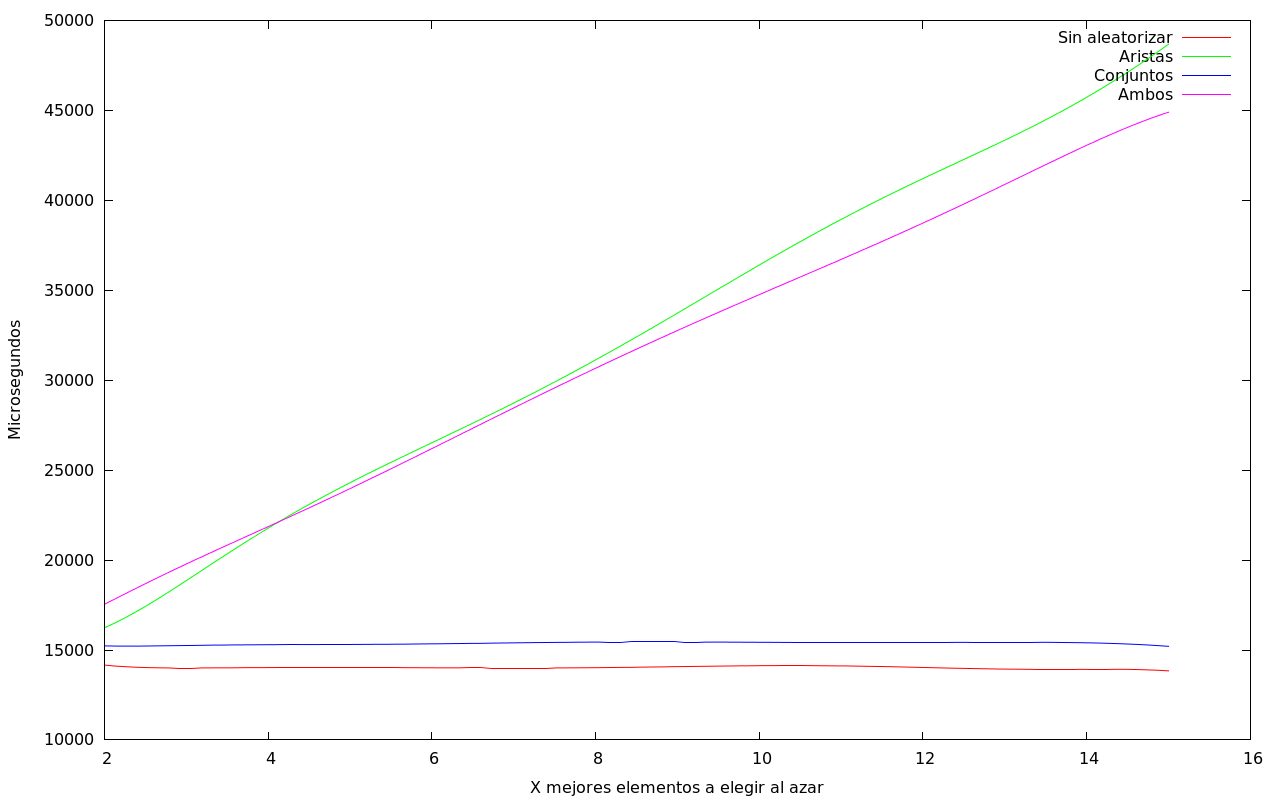
\includegraphics[scale=0.35]{imagenes/grasp-goloso-x-tiempo.png}
  \end{center}
\end{figure}

\vspace*{0.2cm}

Se puede apreciar claramente que, al aleatorizar las aristas, el tiempo crece
linealmente con respecto a la cantidad de elementos a elegir. Esto se debe
a que para elegir al azar entre los mejores, primero se están ordenando todos.

En el caso de la aristas, esto implica ordenar un conjunto de tamaño del orden
de $n^2$. En cambio, los conjuntos están fijos en 15 y ordenarlos en cada
iteración termina pareciendo constante.

Para tener en cuenta en el futuro, este comportamiento se va a mantener en
todos los casos interesantes, ya que si sabemos que van a haber casos con
$k \geq 2m$, simplemente separando todos los nodos de las $m$ aristas en 2
conjuntos distintos nos asegura un peso de 0, y se puede calcular fácilmente.

Esto suma bastante más en el caso de las aristas, ya que (en este caso)
empiezan en 375 y disminuyen de a 1. En cambio, los conjuntos están fijos en
15 y ordenar 15 en cada iteración termina pareciendo constante.

\vspace*{0.5cm}

\begin{figure}[H]
  \begin{center}
    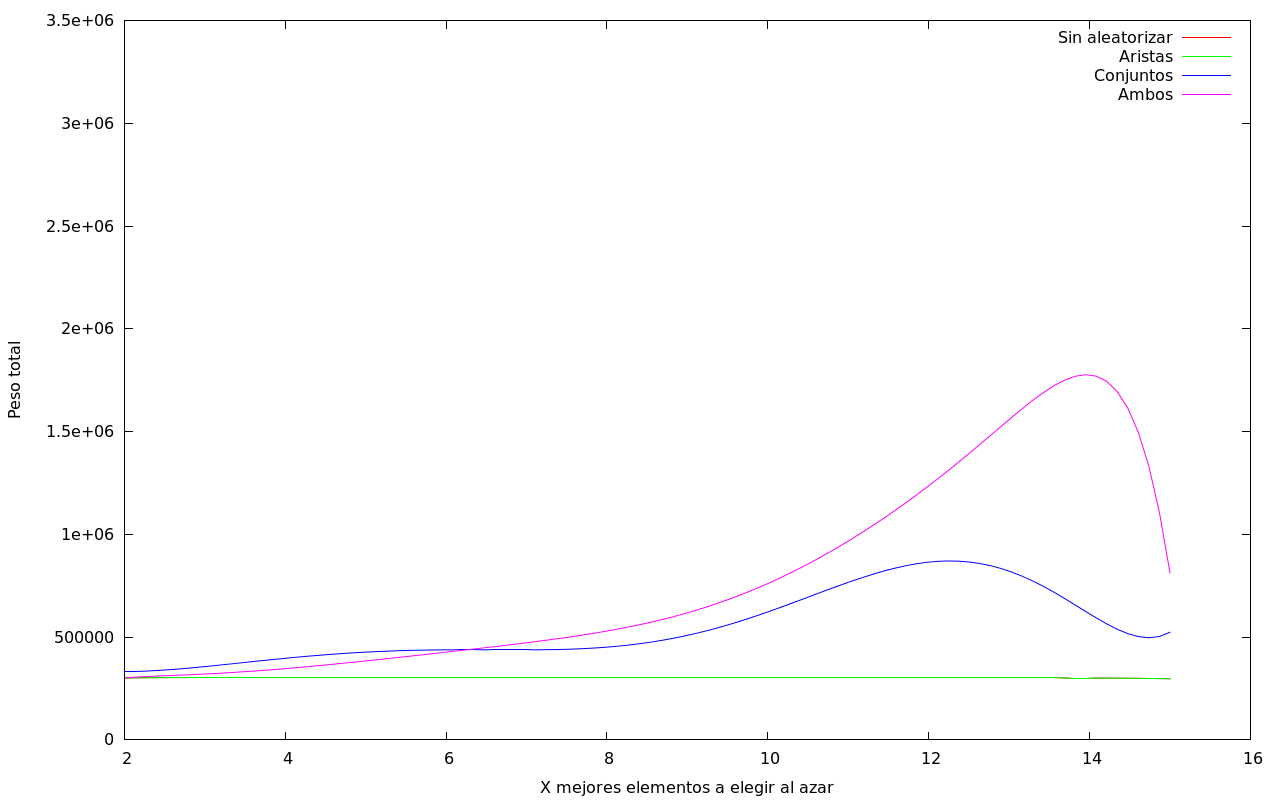
\includegraphics[scale=0.35]{imagenes/grasp-goloso-x-peso.png}
  \end{center}
\end{figure}

\vspace*{0.5cm}

Con respecto al peso, podemos ver que aumenta con respecto al goloso sin
aleatorizar cuando aumenta el $X$. Esto tiene sentido, ya que en el caso $X$
valiendo 15, con $k$ valiendo 15, el algoritmo deja de ser goloso y pasa a ser
totalmente al azar.

Lo que sí se puede observar es que aleatorizar las aristas da un resultado
apenas peor, pero despreciable con respecto a no aleatorizar nada, y no empeora
al aumentar $X$.

\vspace*{0.5cm}

\newpage Veamos si estos comportamientos se mantienen fijando $X$ en 10 (donde el peso total se mantiene relativamente acotado en todas las versiones) y modificando las otras variables.

\begin{figure}[H]
  \begin{center}
    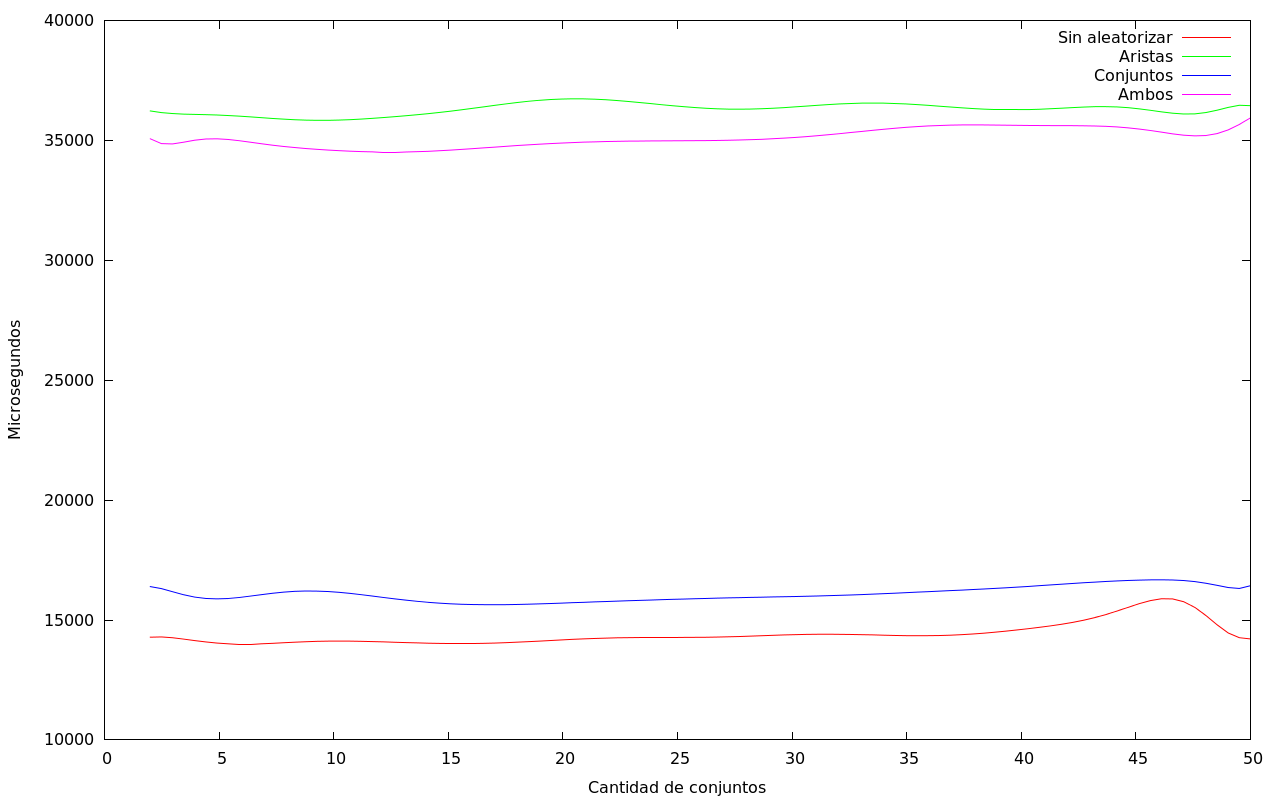
\includegraphics[scale=0.35]{imagenes/grasp-goloso-k-tiempo.png}
  \end{center}
\end{figure}

\begin{figure}[H]
  \begin{center}
    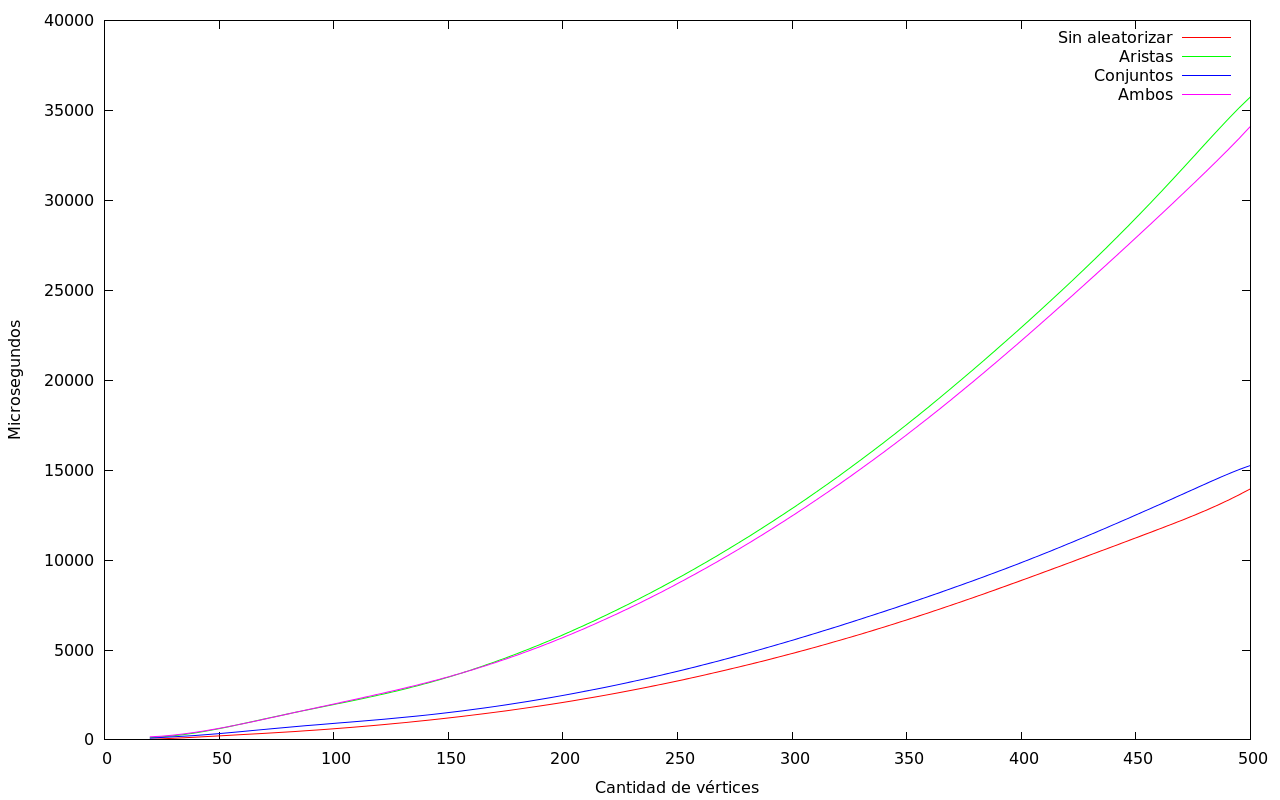
\includegraphics[scale=0.35]{imagenes/grasp-goloso-n-tiempo.png}
  \end{center}
\end{figure}

Podemos observar el mismo comportamiento, con respecto al tiempo, que veníamos
viendo. El tiempo depende de $n$ y aumenta al aleatorizar las aristas (y,
obviamente, cuando se aleatorizan ambos).

\begin{figure}[H]
  \begin{center}
    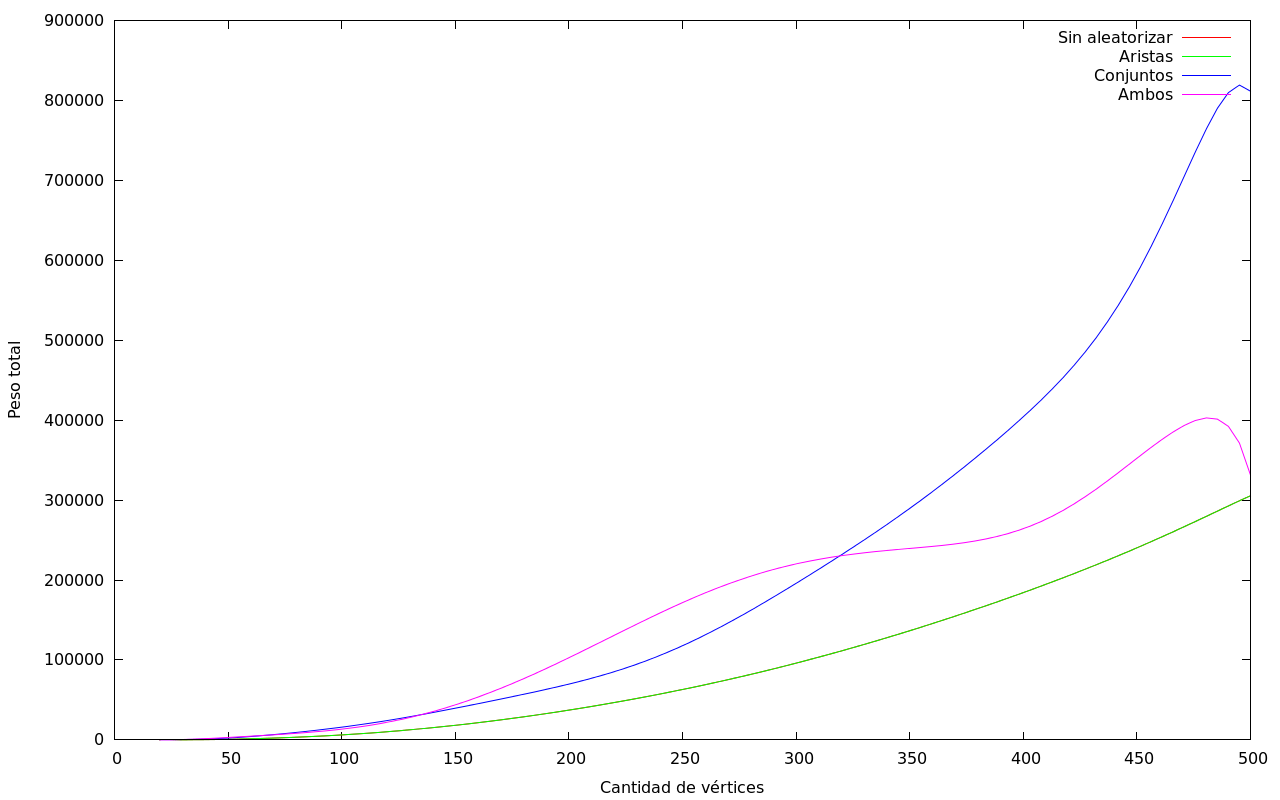
\includegraphics[scale=0.35]{imagenes/grasp-goloso-n-peso.png}
  \end{center}
\end{figure}

\begin{figure}[H]
  \begin{center}
    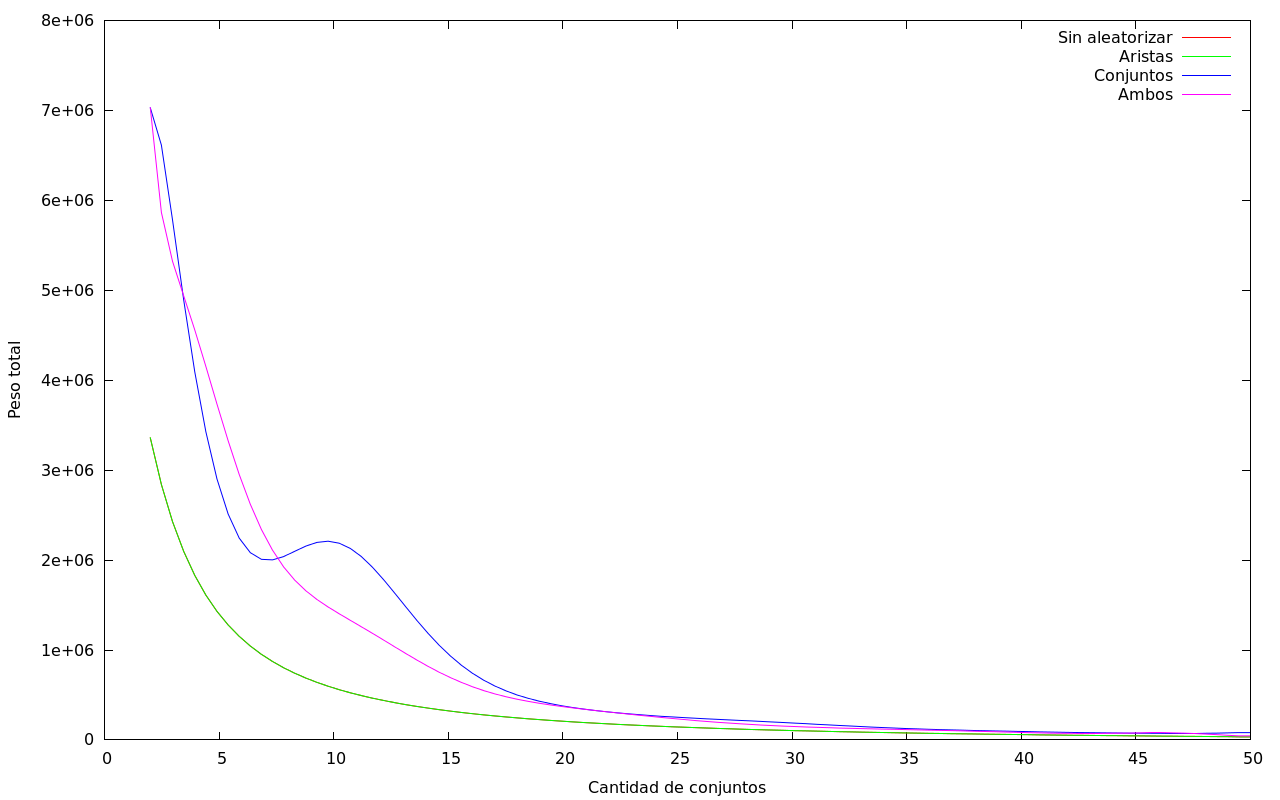
\includegraphics[scale=0.35]{imagenes/grasp-goloso-k-peso.png}
  \end{center}
\end{figure}

Con la calidad también se destacan las mismas situaciones, aleatorizar los
conjuntos genera consistentemente pesos mayores. Y aleatorizar las aristas da
resultados muy similares a no aleatorizar, dando mejores resultados en algunos
casos.

Hasta ahora todo indicaría que si se quiere priorizar tiempos se debería elegir
aleatorizar los conjuntos, pero si se prefiere calidad se debe aleatorizar las
aristas. En ningún caso conviene aleatorizar ambos, ya que sería lo peor de los
dos mundos.

\newpage \subsubsection{Junto a la heurística de búsqueda local}

Sin embargo, si el algoritmo goloso no se ejecuta solo, podría darse que una
estrategia de peores resultados por sí misma, combinada con una búsqueda local,
termine siendo mejor. Por esta razón vamos a ver los mismos casos, pero luego
de aplicarle un algoritmo de búsqueda local.

En el ejercicio identificamos que la heurística \textit{mover} se comporta
mejor que la de \textit{intercambiar}, tanto en calidad de soluciones como en
tiempo de ejecución en todos los casos. Por lo tanto utilizaremos este para las
pruebas.

Comparemos, en primer lugar, los tiempos:

\begin{figure}[H]
  \begin{center}
    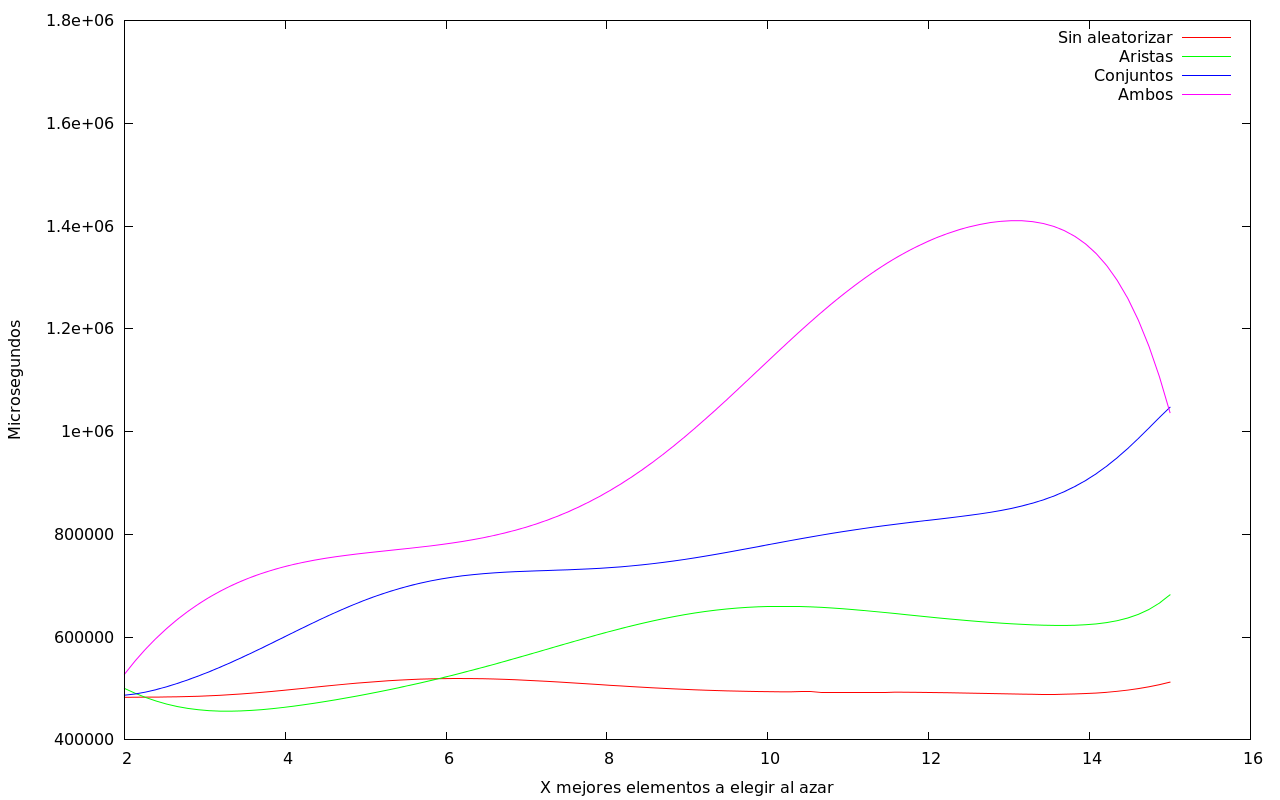
\includegraphics[scale=0.35]{imagenes/grasp-local-x-tiempo.png}
  \end{center}
\end{figure}

\begin{figure}[H]
  \begin{center}
    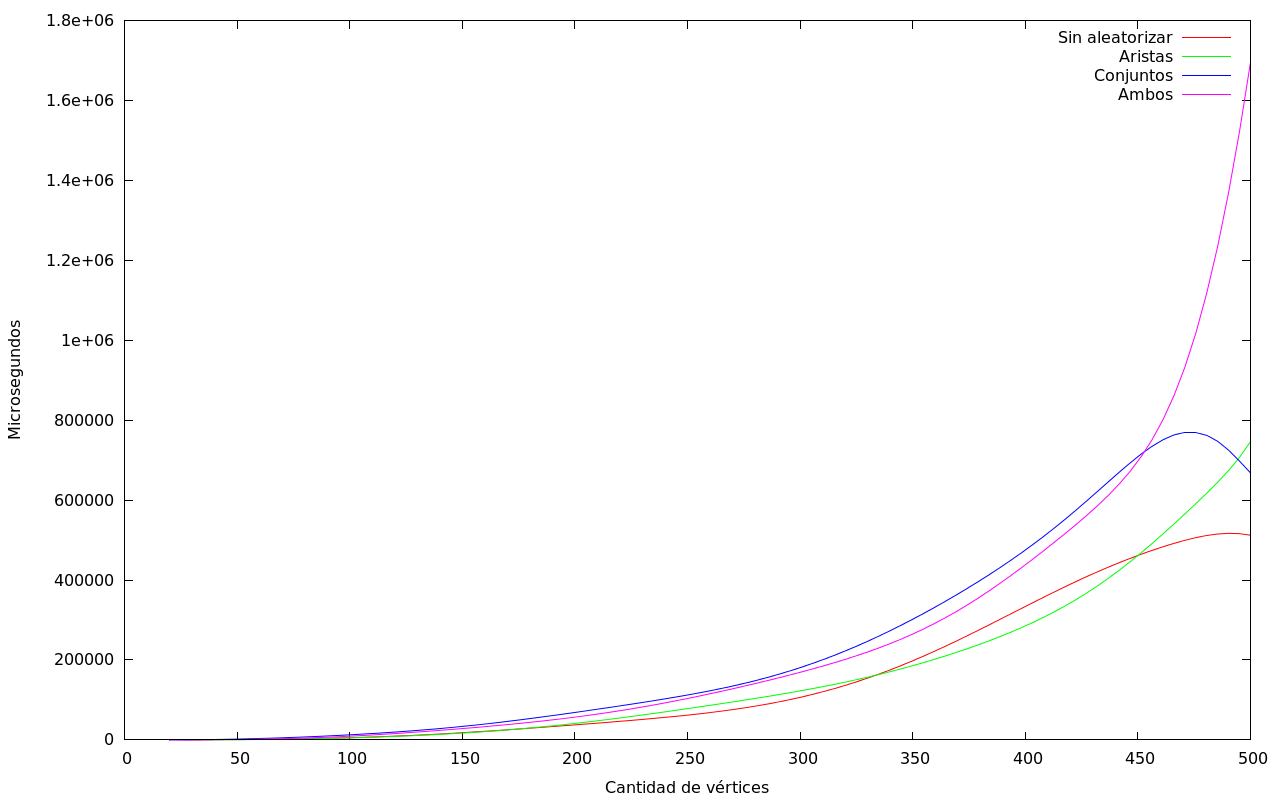
\includegraphics[scale=0.35]{imagenes/grasp-local-n-tiempo.png}
  \end{center}
\end{figure}

\begin{figure}[H]
  \begin{center}
    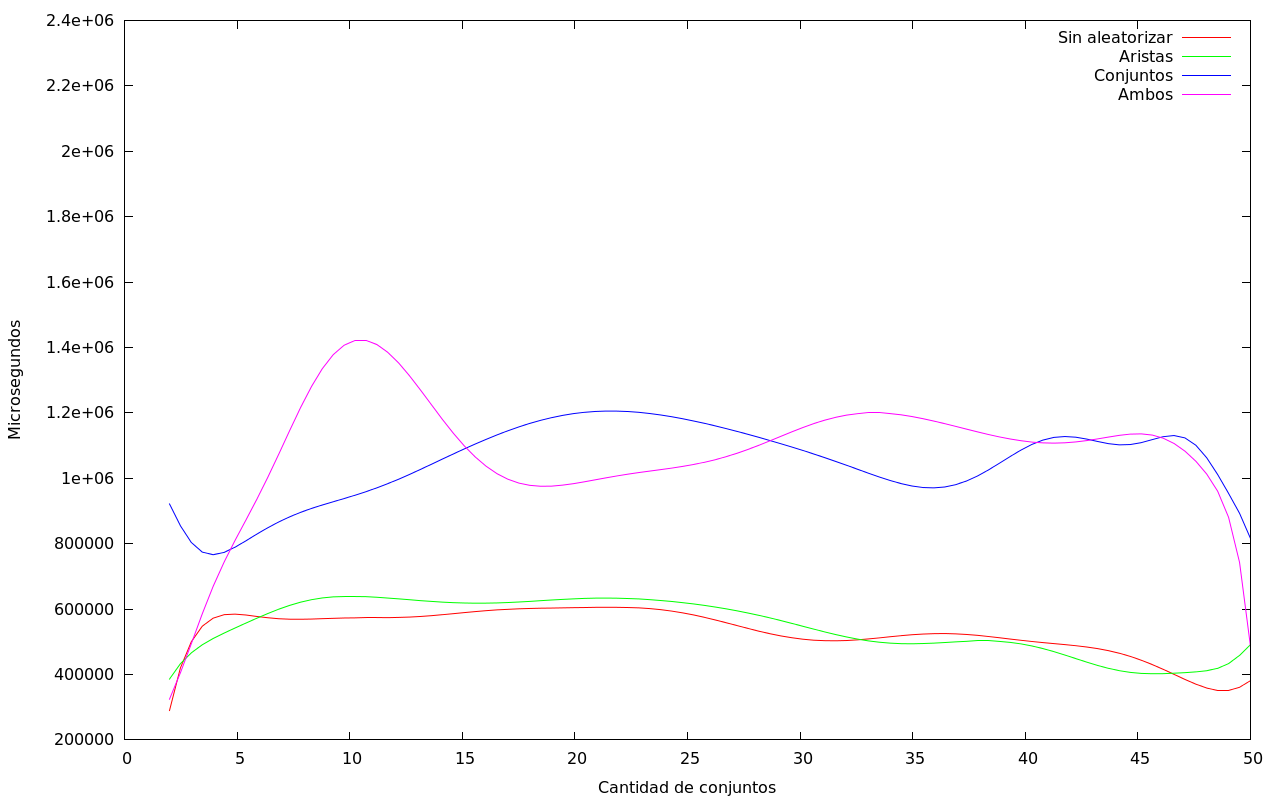
\includegraphics[scale=0.35]{imagenes/grasp-local-k-tiempo.png}
  \end{center}
\end{figure}

Estos experimentos muestran algo bastante particular: aleatorizar por aristas
es lo que menos tiempo demora, a diferencia de lo observado en la
experimentación de la búsqueda local.

En general, los tiempos de todas las versiones redujeron sus diferencias. Se
puede observar que, aunque aleatorizar las aristas sea lo más eficiente, ya no
hay una diferencia creciente entre las otras versiones del algoritmo, todas
se comportan con un orden similar.

Una explicación posible es que con una mejor versión inicial provista por
la heurística golosa, la búsqueda local demora menos en encontrar un mínimo
local.

Ahora veamos la calidad final que obtienen estos algoritmos:


\begin{figure}[H]
  \begin{center}
    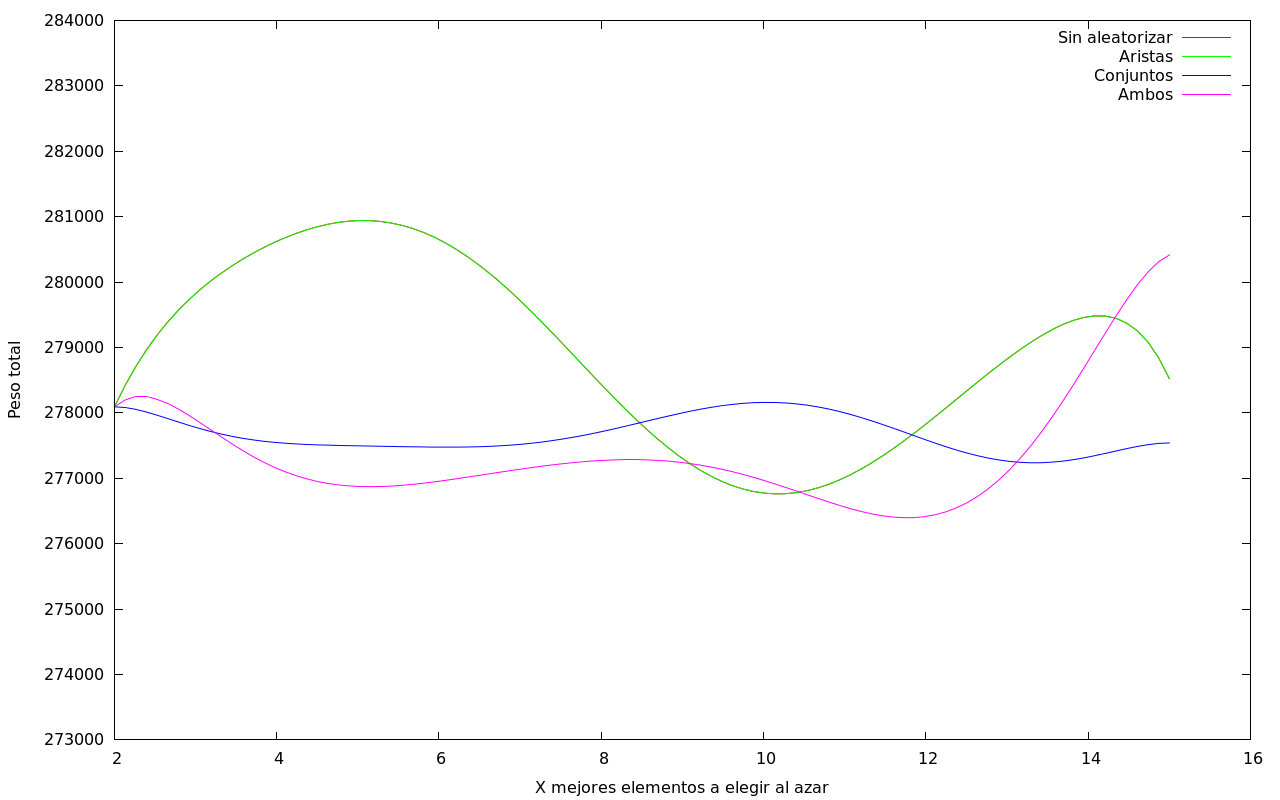
\includegraphics[scale=0.35]{imagenes/grasp-local-x-peso.png}
  \end{center}
\end{figure}

\begin{figure}[H]
  \begin{center}
    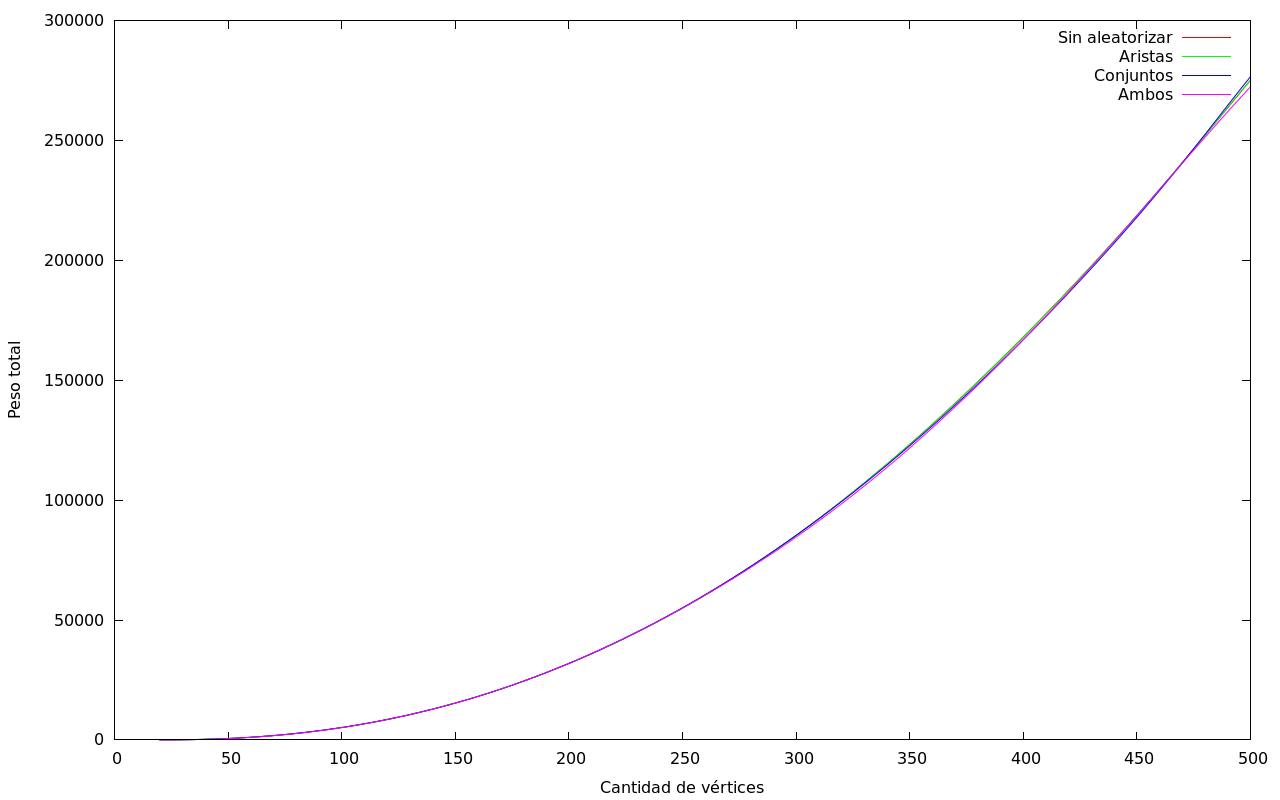
\includegraphics[scale=0.35]{imagenes/grasp-local-n-peso.png}
  \end{center}
\end{figure}

\begin{figure}[H]
  \begin{center}
    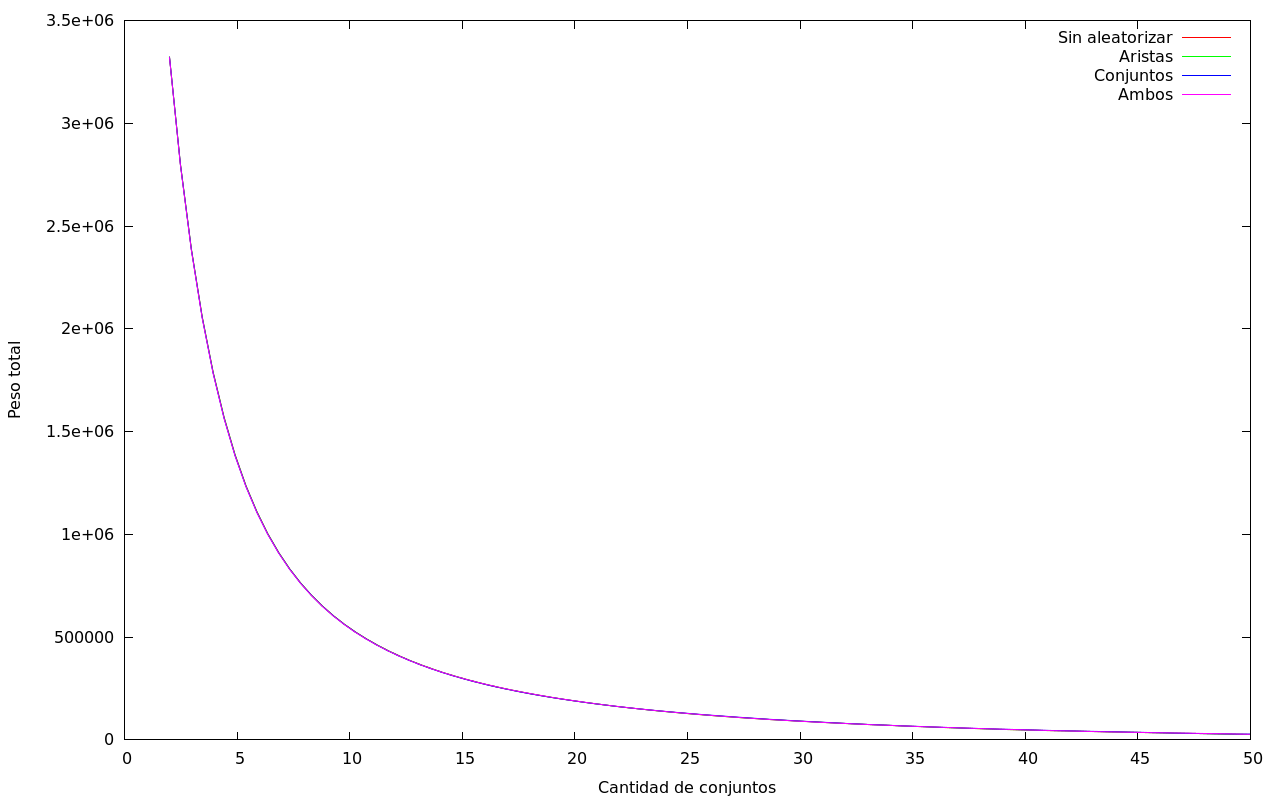
\includegraphics[scale=0.35]{imagenes/grasp-local-k-peso.png}
  \end{center}
\end{figure}

Sorprendentemente, luego de aplicar la búsqueda local, se llega a resultados
similares en todos los casos. En el gráfico que varía $X$ se puede apreciar
que, aunque no son exactamente los mismos resultados, la diferencia es casi
despreciable (menor al 1\% en la mayoría de los casos).

Combinando cualquiera de las variedades de la heurística golosa con la
búsqueda local obtenemos pesos similares, por lo que vamos a usar como
determinante el tiempo.

Consistentemente la utilización de aleatorizar únicamente las aristas dio
mejores tiempos. Por lo tanto, ésta será la utilizada. La cantidad de aristas
al azar a elegir no modifica el tiempo y apenas muy levemente el peso final.
Elegimos utilizar $X$ valiendo 10, ya que dio los mejores resultados combinando
con la búsqueda local y es un número suficientemente grande para dar variedad a
los resultados, pero no tanto que terminen siendo soluciones aleatorias.

\newpage \subsubsection{Criterio de terminación}

Para ver qué criterio de terminación conviene elegir, analizamos ambos contra
un conjunto de de 30 grafos distintos, 15 densos con 200 vértices y 15 completos
con entre 75 y 195 vértices, todos con una partición de 15 conjuntos.

Veamos como se comportan con respecto al tiempo de ejecución:

\vspace*{0.5cm}

\begin{figure}[H]
  \begin{center}
    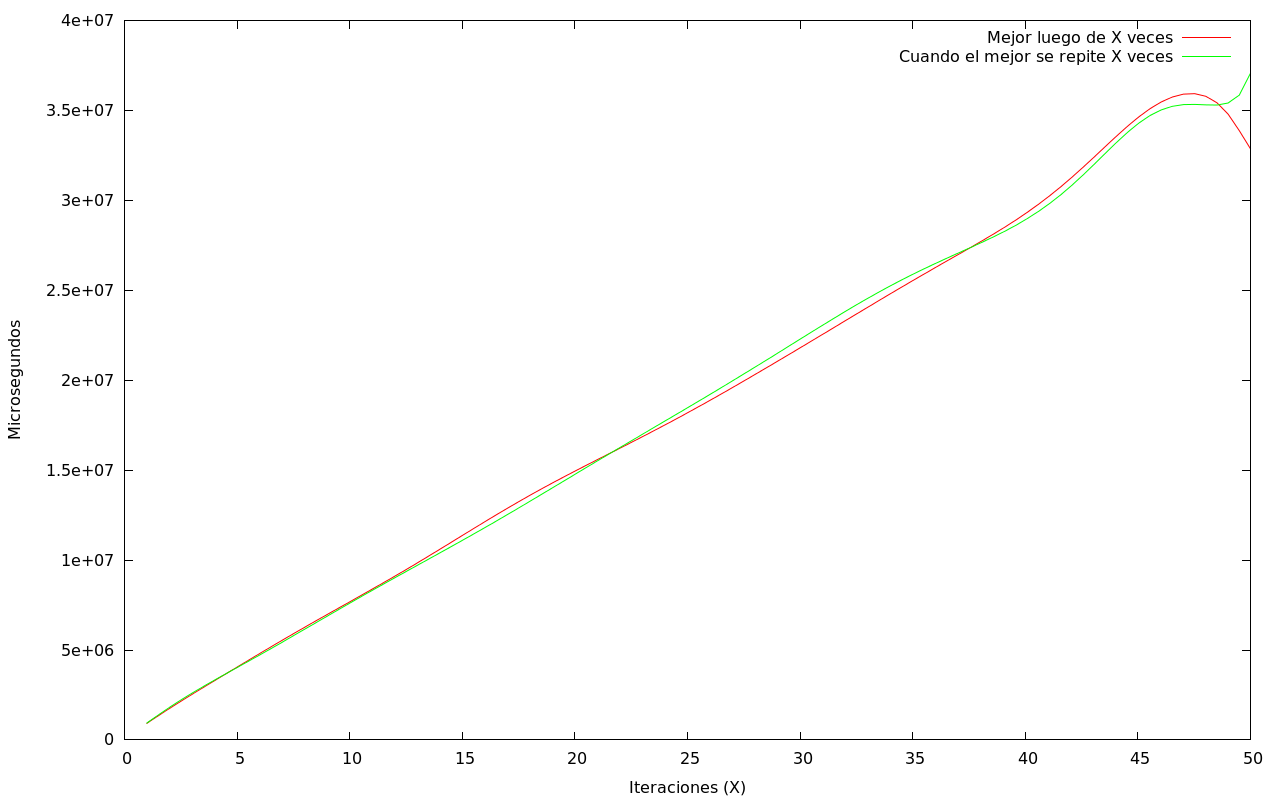
\includegraphics[scale=0.35]{imagenes/grasp-criterio-tiempo.png}
  \end{center}
\end{figure}

\vspace*{0.5cm}

Ambos tienen resultados muy similares, algo que no esperábamos, ya que uno tiene
una cantidad exacta de iteraciones y el otro podría tardar mucho más, ya que
debe encontrar la misma solución varias veces.

Esto significa que, para bien o para mal, está llegando a una misma solución
consistentemente, a pesar de la aleatorización.

Veamos entonces los pesos de las soluciones encontradas:

\vspace*{0.5cm}

\begin{figure}[H]
  \begin{center}
    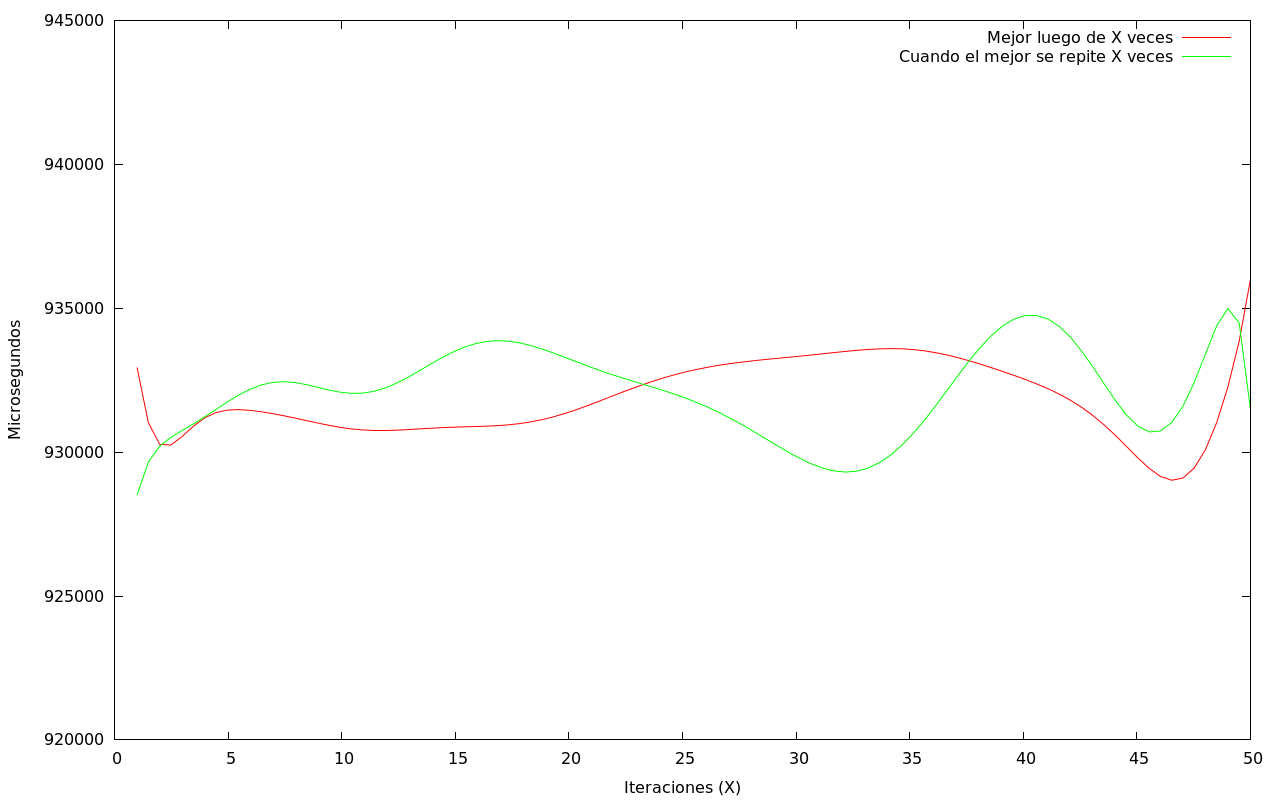
\includegraphics[scale=0.35]{imagenes/grasp-criterio-peso.png}
  \end{center}
\end{figure}

\vspace*{0.5cm}

Analizando estos resultados, no parece haber mucha diferencia, ambos tienen
resultados muy similares. Tampoco parecen reducir mucho el peso al
aumentar las repeticiones.

Elegimos quedarnos con el criterio de cuando el mejor se repita $X$ veces, con
$X = 34$, y con el criterio de parar luego de X veces con $X = 47$, siendo que
ambos dieron los mejores resultados, pero no es evidente que uno sea mejor que
el otro.
